\documentclass[10pt,a4paper]{article}
\usepackage[a4paper,margin=1.8cm,top=1.6cm,bottom=1.8cm]{geometry}
\usepackage[T1]{fontenc}
\usepackage{newtxtext,newtxmath}
\usepackage{microtype}
\usepackage{graphicx}
\usepackage{booktabs}
\usepackage[font=small,labelfont=bf,skip=3pt]{caption}
\usepackage[hidelinks]{hyperref}
\usepackage{enumitem}
\usepackage{titlesec}
\usepackage{xcolor}

\titleformat{\section}{\normalsize\bfseries}{\thesection}{0.5em}{}
\titlespacing*{\section}{0pt}{7pt}{3pt}
\setlist{nosep,leftmargin=1.3em}
\setlength{\parskip}{2.5pt}
\setlength{\parindent}{0pt}
\setlength{\textfloatsep}{8pt}
\setlength{\floatsep}{6pt}
\renewcommand{\topfraction}{0.85}
\renewcommand{\bottomfraction}{0.5}
\renewcommand{\textfraction}{0.08}
\setcounter{totalnumber}{4}

\newcommand{\etaA}{\eta_A}
\newcommand{\etaB}{\eta_B}

\begin{document}

\begin{center}
{\large\bfseries Does LoRA+ transfer to vision--language models?\\[1pt]
Learning-rate ratios for LoRA finetuning of SmolVLM-256M}\\[4pt]
{\small EN4554 Deep Learning for Vision --- Assignment 1, Part 1}\\[1pt]
{\small De Zoysa A.\,S.\,I. (220106D) \quad$\cdot$\quad Jayasekara S.\,P.\,R. (220257N)}
\end{center}
\vspace{-4pt}
\suppressfloats[t]

\section{Central claim of the paper}
LoRA+ (Hayou, Ghosh \& Yu, ICML 2024) argues, from an infinite-width scaling analysis, that training the LoRA
adapter matrices $A$ and $B$ with the \emph{same} learning rate gives inefficient feature learning in wide models.
Setting $\etaB=\lambda\,\etaA$ with a fixed $\lambda\gg1$ is claimed to improve accuracy by 1--2\% and finetuning
speed by up to ${\sim}2\times$ at the same cost as LoRA.

\section{Concept translated and the supporting evidence in the paper}
\begin{itemize}
\item \textbf{Off-diagonal optimum (main concept).} Figs.~3 and 4 sweep $(\etaA,\etaB)$ for RoBERTa-base and GPT-2 on GLUE.
Test accuracy is maximal for $\etaB\gg\etaA$, above the best near-equal setting ($\etaB/\etaA\in[1,1.25]$, marked in red).
\item \textbf{Speed-up.} Fig.~7: with $\lambda=2^4$, test accuracy rises roughly $2\times$ faster than with $\etaB=\etaA$ (RoBERTa, MNLI).
\item \textbf{Harder tasks.} Sec.~5.1: the gap to $\etaA\approx\etaB$ is ``more pronounced for `harder' tasks like MNLI and QQP''.
\end{itemize}
For the initialisation used by \texttt{peft} ($B=0$, the paper's \texttt{Init[1]}), Sec.~5.3 reports an optimal $\lambda$ of order $2^2$--$2^3$.

\section{Translated hypotheses}
\textbf{H1 (accuracy).} When LoRA-finetuning a small VLM for VQA, the best accuracy over an $(\etaA,\lambda)$ grid lies at
$\lambda>1$, and the best LoRA+ setting beats the best equal-learning-rate LoRA setting.
\textbf{H1s (speed).} For the same compute, LoRA+ reaches a given loss or accuracy in fewer steps.
\textbf{H2 (harder task).} The LoRA+ gain is larger on the task that is harder for the model: TextVQA, which requires reading
text in images (zero-shot 32.8\%), versus VQAv2 (45.3\%).

\section{Experimental setup}
\textbf{Model.} SmolVLM-256M-Instruct (256.5M parameters): a SigLIP vision encoder (12 layers, width 768) and a
SmolLM2-135M language model (30 layers, width 576). Images are resized to $512{\times}512$ with tiling disabled
(64 visual tokens), which keeps a full grid affordable on a free T4. The model's default instead tiles images up to
2048\,px (${\approx}870$ tokens); Sec.~5 measures what this choice costs. \textbf{Adapters.} LoRA $r=\alpha=8$ (as in the
paper's Figs.~3--4), dropout 0, on every attention ($q,k,v,o$) and MLP projection of \emph{both} towers: 282 modules,
3.77M trainable parameters (1.45\%). LoRA+ uses two AdamW parameter groups, all $A$ at $\etaA$ and all $B$ at
$\lambda\etaA$. Everything else is identical across runs.
\textbf{Data.} TextVQA and VQAv2 (\texttt{lmms-lab} copies). For each, 2{,}000 training questions from the official
\emph{train} split (1{,}719 / 1{,}144 images) and 500 evaluation questions from the official \emph{validation} split
(439 / 393 images), sampled with seed 42. The prompt asks for ``a single word or phrase''. The training target is the most
frequent of the 10 human answers, and the loss is computed on the answer tokens only.
\textbf{Training.} Batch 16, 2 epochs (250 steps), 6\% linear warm-up then linear decay, gradient clipping 1.0, weight
decay 0, fp16 mixed precision (fp32 adapters). \textbf{Metric.} Official VQA accuracy (10 answers, standard
normalisation), greedy decoding.
\textbf{Protocol.} (i)~A grid with seed 42: $\etaA\in\{1,2,4,8,16\}\times10^{-4}$, and $\lambda\in\{1,2,4,8,16,32\}$
(TextVQA) or $\{1,4,16\}$ (VQAv2), giving 45 runs. (ii)~Seven key settings re-run with three \emph{fresh} seeds
$\{1,2,3\}$ (21 runs), with accuracy on the first 200 evaluation questions logged during training. Fresh seeds remove the
optimistic bias of reporting the run that was used for selection. (iii)~A resolution test: zero-shot on the same
500 questions, re-loaded from the full-resolution originals, at five input settings (Table~\ref{tab:res}).
(iv)~Differences are tested with a paired bootstrap (20k resamples) over the 500 questions, using per-question scores
averaged over seeds. Between-task differences resample each task independently.

\begin{figure}[t]
\centering
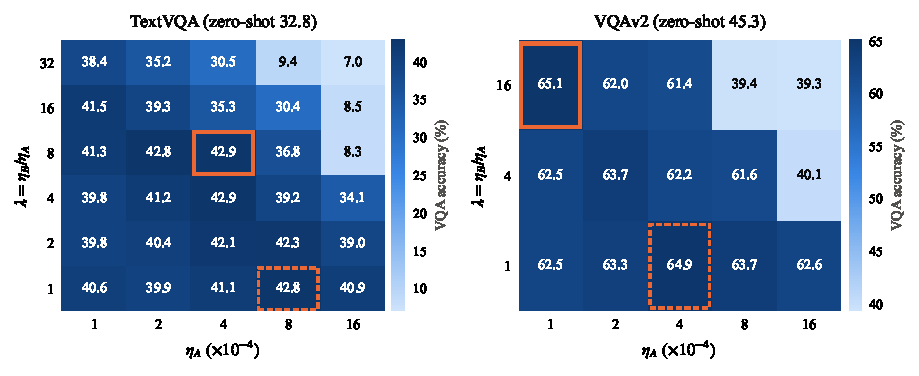
\includegraphics[width=\linewidth]{figs/fig1_heatmaps.pdf}
\caption{Accuracy over the learning-rate grid (seed 42, 500 eval questions). The bottom row ($\lambda=1$) is plain LoRA.
Solid box: best overall. Dashed box: best plain LoRA. The optimum is a broad plateau over $\lambda\in[1,8]$, not a peak
at $\lambda>1$. Failure is set by $\etaB=\lambda\etaA$: every run with $\etaB\ge1.3\times10^{-2}$ ends below
zero-shot whatever $\lambda$ is, and on TextVQA the decline starts at $\etaB=6.4\times10^{-3}$.}
\label{fig:grid}
\end{figure}

\section{Results and interpretation}
\textbf{Baseline vs.\ adapted.} Finetuning is clearly effective. Tuned LoRA improves on zero-shot by
$+8.3$ [$+4.7,+12.0$] points on TextVQA and $+18.2$ [$+14.1,+22.2$] on VQAv2 (Table~\ref{tab:main}).

\textbf{H1 (accuracy): not supported.} In the seed-42 grid (Fig.~\ref{fig:grid}), the best LoRA+ cell beats the best LoRA
cell by only $+0.1$ (TextVQA) and $+0.3$ (VQAv2) points. The best accuracy per $\lambda$ row is flat for TextVQA
(42.8, 42.3, 42.9, 42.9, 41.5, 38.4 for $\lambda=1\ldots32$). With fresh seeds the small advantage disappears
(Table~\ref{tab:main}). Tuned LoRA+ is $-1.7$ [$-3.7,+0.3$] points \emph{below} tuned LoRA on TextVQA (lower in all three
seeds) and $-0.0$ [$-1.7,+1.6$] on VQAv2. This is a \emph{winner's curse}: the settings picked as best on seed 42 lost
more on fresh seeds (LoRA+ TextVQA $42.9\to39.4$) than settings that were not picked (LoRA, $\eta=10^{-4}$:
$40.6\to40.1$). LoRA+ had 25 grid cells to select from, LoRA only 5.

\begin{table}[t]
\centering\small
\caption{Fresh-seed results (seeds 1--3, mean $\pm$ s.d.; 500 eval questions). ``Steps'': training steps until the
10-step mean loss drops below 1.0. $\Delta$: LoRA+ minus the LoRA row named in brackets, from a paired bootstrap
95\% CI. On VQAv2 the tuned LoRA+ setting coincides with $\etaA=10^{-4},\lambda=16$.}
\label{tab:main}
\setlength{\tabcolsep}{5pt}
\begin{tabular}{@{}llccccl@{}}
\toprule
Task & Setting & $\etaA$ & $\lambda$ & Accuracy (\%) & Steps & $\Delta$ vs.\ LoRA (95\% CI) \\
\midrule
TextVQA & zero-shot & -- & -- & 32.8 & -- & \\
 & LoRA, tuned $\eta$ & $8\!\times\!10^{-4}$ & 1 & \textbf{41.1} $\pm$ 0.7 & 20 & \\
 & LoRA+, tuned & $4\!\times\!10^{-4}$ & 8 & 39.4 $\pm$ 0.3 & 15 & $-1.7$ [$-3.7$, $+0.3$] (tuned) \\
 & LoRA, $\eta=10^{-4}$ & $1\!\times\!10^{-4}$ & 1 & 40.1 $\pm$ 0.5 & 35 & \\
 & LoRA+, same $\etaA$ & $1\!\times\!10^{-4}$ & 16 & 40.7 $\pm$ 0.8 & 16 & $+0.6$ [$-1.5$, $+2.7$] (same $\etaA$) \\
\midrule
VQAv2 & zero-shot & -- & -- & 45.3 & -- & \\
 & LoRA, tuned $\eta$ & $4\!\times\!10^{-4}$ & 1 & \textbf{63.4} $\pm$ 0.9 & 13 & \\
 & LoRA+, tuned & $1\!\times\!10^{-4}$ & 16 & \textbf{63.4} $\pm$ 0.3 & \textbf{7} & $-0.0$ [$-1.7$, $+1.6$] (tuned) \\
 & LoRA, $\eta=10^{-4}$ & $1\!\times\!10^{-4}$ & 1 & 62.8 $\pm$ 0.8 & 37 & $+0.7$ [$-1.4$, $+2.7$] (same $\etaA$) \\
\bottomrule
\end{tabular}
\end{table}

\begin{figure}[b]
\centering
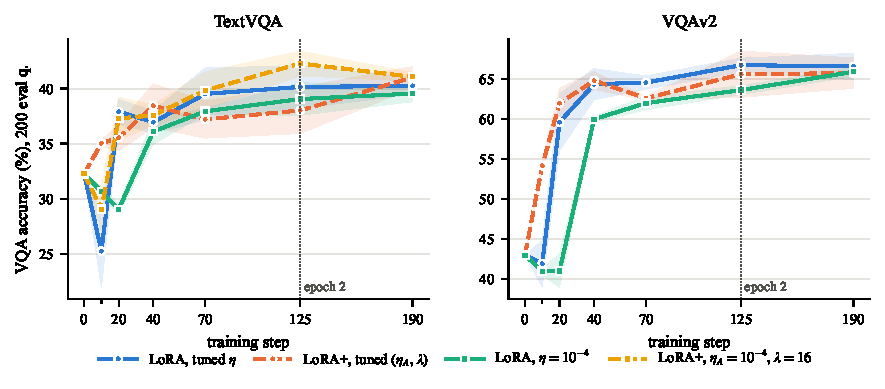
\includegraphics[width=\linewidth]{figs/fig2_curves.pdf}
\caption{Accuracy during training (200 eval questions; mean of 3 fresh seeds, band $=\pm$1 s.d.; step 0 = zero-shot).
LoRA+ (dashed) adapts fastest at the start but ends level with tuned LoRA (solid). The steps after the dotted line are
the second epoch over the same questions.}
\label{fig:curves}
\end{figure}

\textbf{H1s (speed): supported.} At the same $\etaA=10^{-4}$, LoRA+ reaches a training loss below 1.0 in $2.2\times$
fewer steps on TextVQA (35$\to$16) and $5\times$ fewer on VQAv2 (37$\to$7). Even against tuned LoRA it is faster on VQAv2
(13$\to$7, close to the paper's ${\sim}2\times$). After 10 steps its VQAv2 accuracy is 54.1\% versus 41.9\% for tuned
LoRA (Fig.~\ref{fig:curves}). The advantage is gone well before step 250.
\emph{Mechanism.} With $B=0$ at initialisation, $\partial L/\partial A\propto B^{\top}=0$, so the first updates move
only $B$, and early progress is set by $\etaB$. LoRA+ raises $\etaB$ without raising $\etaA$. This also explains why the
stability boundary in Fig.~\ref{fig:grid} depends on $\etaB$. For a fixed $\etaB$, a smaller $\etaA$ is better: at
$\etaB=3.2\times10^{-3}$, $\etaA=4\times10^{-4}$ gives 42.9 versus 38.4--39.3 for the other cells. This agrees with
``$B$ tolerates a larger rate than $A$''. But plain LoRA recovers the same speed simply by raising its single $\eta$,
so with a tuned $\eta$ and our budget both converge to the same accuracy.

\textbf{H2 (harder task): not supported.} The LoRA+ gain on TextVQA minus that on VQAv2 is $-1.7$ [$-4.3,+0.9$], so the
sign is opposite to the prediction.

\begin{table}[t]
\centering\small
\caption{Zero-shot accuracy (\%) vs.\ visual input, on the same 500 questions per task re-loaded from the
full-resolution originals. Brackets: change vs.\ 512\,px, paired 95\% CI. ``Tiles'' is SmolVLM's global view plus
512\,px tiles; 2048\,px is the model's default. (At 512\,px this pipeline gives 31.6 / 45.3, against 32.8 / 45.3 from the
512\,px copies in Table~\ref{tab:main}.) Last row: our finetuned models, which see only the 64-token input.}
\label{tab:res}
\setlength{\tabcolsep}{5pt}
\begin{tabular}{@{}lcll@{}}
\toprule
Visual input & Tokens & TextVQA & VQAv2 \\
\midrule
256\,px, no tiling & 64 & 28.4 \;($-3.3$ [$-6.7$, $+0.1$]) & 43.7 \;($-1.6$ [$-4.7$, $+1.4$]) \\
512\,px, no tiling (our training input) & 64 & 31.6 & 45.3 \\
tiles, longest edge 1024\,px & ${\approx}320$ & 48.8 \;($+17.2$ [$+13.3$, $+21.2$]) & 64.3 \;($+19.0$ [$+14.9$, $+23.2$]) \\
tiles, longest edge 1536\,px & ${\approx}570$ & 50.6 \;($+19.0$ [$+15.1$, $+22.9$]) & 65.0 \;($+19.7$ [$+15.7$, $+23.7$]) \\
tiles, longest edge 2048\,px (default) & ${\approx}870$ & 49.1 \;($+17.5$ [$+13.5$, $+21.5$]) & 64.4 \;($+19.1$ [$+15.0$, $+23.2$]) \\
\midrule
LoRA finetuned, 512\,px, no tiling & 64 & 41.1 & 63.4 \\
\bottomrule
\end{tabular}
\end{table}

\textbf{Bonus: a vision-specific interpretation, tested.} Unlike the paper's text tasks, a VLM task can be hard for two
separate reasons: the model must \emph{adapt} (answer format, task skills), or the visual tokens lack the
\emph{information} (perception). A learning-rate ratio can only act on the first. We separated the two by changing only
the visual input, zero-shot (Table~\ref{tab:res}). The simplest version of the idea, that TextVQA alone is
perception-limited, was tested with two predictions fixed before the run: halving the resolution should hurt TextVQA
more (P1), and the model's default tiling should help it more (P2). \emph{Both fail.} At a fixed 64 tokens, 256\,px instead
of 512\,px costs only $-3.3$ and $-1.6$ points (P1: $-1.7$ [$-6.2,+3.0$]), so pixels are not the binding constraint.
Tiling ($5$--$14\times$ more tokens) adds $+17$ to $+20$ points on \emph{both} tasks, with no clear further gain beyond
${\approx}320$ tokens (P2: $-1.6$ [$-7.3,+4.1$]). The token budget limits both tasks equally, so a TextVQA-specific
perception bottleneck is rejected.

\textbf{What separates the tasks: can finetuning stand in for detail? (post-hoc, exploratory).} On VQAv2, LoRA at 64 tokens recovers
95\% of the tiling gain (default tiling minus LoRA: $+1.0$ [$-2.4,+4.4$]). Among questions the 512\,px zero-shot model
gets wrong, tiling and LoRA fix largely the \emph{same} ones ($\phi=0.51$ between ``fixed by tiling'' and ``fixed by
LoRA''). On TextVQA, LoRA recovers only 48\% ($+8.0$ [$+3.8,+12.3$]; between-task difference $+7.1$ [$+1.5,+12.5$]), and
the two fix largely \emph{different} questions ($\phi=0.20$; difference $+0.31$ [$+0.15,+0.47$]). The conclusion is
the same for every tiled setting and score threshold. Typical among the 67 TextVQA questions fixed only by tiling are misreadings
(jersey ``3''$\to$``6'', tail number ``ANA''$\to$``JA617A''). So on VQAv2 the low-token deficit behaves like an
\emph{adaptation} problem, which an adapter learns. On TextVQA about half of it behaves like missing visual
\emph{information}, which our adapters on the same 64 tokens did not recover, whatever the learning-rate ratio. This is
consistent with H2 failing but does not prove the link.

\textbf{Future work.} The direct test is to repeat LoRA vs.\ LoRA+ with tiling on (${\approx}5\times$ the compute). A further VLM-specific extension follows from the theory: the optimal $\lambda$
should scale with width, and the two towers differ (768 vs.\ 576), which suggests a per-tower $\lambda$ (untested).

\textbf{Limitations.} One small model. 2{,}000-question subsets and 250 steps. One 500-question evaluation set per task,
shared by selection and confirmation (mitigated by fresh seeds and paired tests). All finetuning used the cheap 64-token
input, which Table~\ref{tab:res} shows costs ${\sim}18$ points. The substitution analysis was designed after seeing P1/P2.
The pretraining data of SmolVLM may include the train splits of these datasets.

\textbf{Conclusion.} LoRA+'s \emph{optimisation-speed} claim transfers to a 256M-parameter VLM: faster early adaptation,
up to ${\sim}2\times$ against tuned LoRA. Its \emph{accuracy} claim and its ``larger gains on harder tasks'' claim do not
transfer once plain LoRA's learning rate is tuned and results are confirmed on fresh seeds. For this VLM the visual
token budget moves accuracy by ${\sim}18$ points, against ${\le}2$ for the learning-rate ratio, and finetuning can stand
in for missing visual detail on VQAv2 (95\%) but only about half-way on TextVQA (48\%). \textit{Code:}
\texttt{01\_setup\_data\_zeroshot}, \texttt{02\_lora\_vs\_loraplus\_grid}, \texttt{03\_seed\_repeats},
\texttt{04\_resolution\_test} (Colab T4) produce all results. \texttt{05\_report\_numbers} (CPU) recomputes every number
in this report from them.

\end{document}
